\subsection{Đề 2}
\Opensolutionfile{ans}[ans/ans-CTST_1-OTGK1_De2-LC]
\caulc
\begin{ex}%[1D1N1-3]
	\immini[thm]{Xác định số đo của góc lượng giác được biểu diễn trong hình bên.
		\choice
		{$-765^\circ$}
		{\True$-675^\circ$}
		{$765^\circ$}
		{$675^\circ$}
		}
		{
		\begin{tikzpicture}[scale=1, font=\footnotesize, line join=round, line cap=round, >=stealth,thick]
			\path
			(0:0) coordinate (O)
			(0:2) coordinate (u)
			(45:2) coordinate (v)	;
			\draw	(u)--(O)--(v);
			\draw pic["\tiny$45^\circ$",draw,angle eccentricity=1.8,angle radius=0.35cm]{angle=u--O--v};
			\draw[samples=200,->,red,thick] plot[domain=0:-360*2+45](\x:1+\x/2500);
			\foreach \x/\y in {u/-80, v/180,O/-100}{\fill (\x) circle(0pt) ($(\x)+(\y:0.25cm)$) node{$\x$};}
		\end{tikzpicture}
	}
	\loigiai{
		Số đo của góc lượng giác $(Ou,Ov)$ trên hình bằng $-2\cdot360^\circ+45^\circ=-675^\circ$.
	}
\end{ex}
\begin{ex}%[1D1N2-2]
	Cho $\pi <\alpha<\dfrac{3\pi}{2}$. Khẳng định nào sau đây là đúng?
	\choice
	{$\sin \alpha >0$}
	{$\cos \alpha >0$}
	{\True $\sin \left(\dfrac{\pi}{2}-\alpha\right) <0$}
	{$\cos \left(\dfrac{\pi}{2}-\alpha\right) >0$}
	\loigiai{Ta có $\pi <\alpha<\dfrac{3\pi}{2}$ nên $\sin \alpha <0$ và $\cos \alpha <0$.\\
		Mà $\sin \left(\dfrac{\pi}{2}-\alpha\right) =\cos \alpha<0$ nên
		$\cos \left(\dfrac{\pi}{2}-\alpha\right) =\sin \alpha<0$.
	} 
\end{ex}
\begin{ex}%[1D1N3-1]
	Trong các mệnh đề sau, mệnh đề nào là mệnh đề \textbf{sai}?
	\choice
	{$\sin a+\sin b=2\sin \dfrac{a+b}{2}\cos \dfrac{a-b}{2}$}
	{\True $\cos a-\cos b=2\sin \dfrac{a+b}{2}\sin \dfrac{a-b}{2}$}
	{$\cos a+\cos b=2\cos \dfrac{a+b}{2}\cos \dfrac{a-b}{2}$}
	{$\sin a-\sin b=2\cos \dfrac{a+b}{2}\sin \dfrac{a-b}{2}$}
	\loigiai{
		Công thức đúng là $\cos a-\cos b=-2\sin \dfrac{a+b}{2}\sin \dfrac{a-b}{2}$.}
\end{ex}

\begin{ex}%[1D1N4-1]
	Tập giá trị của hàm số $y= \cos x$ là tập hợp nào sau đây?
	\choice
	{$[0; +\infty]$}
	{$\mathbb{R}$}
	{$(-\infty; 0]$}
	{\True $ [-1; 1]$}
	\loigiai{
		Với mọi $x \in \mathbb{R}$ thì $-1 \leq \cos x \leq 1$.
	}
\end{ex}
\begin{ex}%[1D1N5-3]
	Phương trình $\cos x=\cos\dfrac{\pi}{15}$ có nghiệm là
	\choice
	{$x=\pm\dfrac{\pi}{15}+k\pi$, $k\in\mathbb{Z}$}
	{\True $x=\pm \dfrac{\pi}{15}+k2\pi$, $k\in\mathbb{Z}$}
	{$\hoac{&x=\dfrac{\pi}{15}+k\pi\\&x=\dfrac{14\pi}{15}+k\pi}$, $k\in\mathbb{Z}$}
	{$\hoac{&x=\dfrac{\pi}{15}+k2\pi\\&x=\dfrac{14\pi}{15}+k2\pi}$, $k\in\mathbb{Z}$}
	\loigiai{
		Ta có
		$\cos x=\cos\dfrac{\pi}{15}\Leftrightarrow x=\pm \dfrac{\pi}{15}+k2\pi$,  $k\in\mathbb{Z}$.
	}
\end{ex}
\begin{ex}%[1D2N1-3]
	Cho dãy số $(u_n)$ có $u_n=\dfrac{2n-1}{n+1}$. Tính $u_8$.
	\choice
	{\True $u_8=\dfrac{5}{3}$}
	{$u_8=\dfrac{11}{9}$}
	{$u_8=\dfrac{17}{9}$}
	{$u_8=1$}
	\loigiai
	{
		Ta có $u_8=\dfrac{2\cdot 8-1}{8+1}=\dfrac{5}{3}$.
	}
\end{ex}
\begin{ex}%[1D2N2-2]
	Dãy nào sau đây là cấp số cộng?
	\choice
	{$1$; $5$; $9$; $5$; $1$}
	{$1$; $3$; $5$; $7$; $11$}
	{\True $2$; $5$; $8$; $11$}
	{$3$; $7$; $3$; $7$}
	\loigiai{
		Dãy số $2$; $5$; $8$; $11$ là một cấp số cộng với công sai $d=3$.
	}
\end{ex}
\begin{ex}%[1D2N3-6]
	Cho cấp số nhân $(u_n)$ có số hạng đầu $u_1=3$ và công bội $q=2$. Tổng của $10$ số hạng đầu tiên của cấp số nhân đó bằng
	\choice
	{$\dfrac{1023}{2}$}
	{$1023$}
	{$1536$}
	{\True $3069$}
	\loigiai{
		Ta có	$S_{10}=u_1\cdot \dfrac{1-q^{10}}{1-q}=3\cdot \dfrac{1-2^{10}}{1-2}=3069$.
	}
\end{ex}
\begin{ex}%[1D1H5-3]
	Giải phương trình $\sin x=\dfrac{\sqrt{3}}{2}$.
	\choice
	{$x= \pm \dfrac{\pi}{3}+k 2 \pi$, $k\in\mathbb{Z}$}
	{$x=\dfrac{\pi}{3}+k \pi$, $k\in\mathbb{Z}$}
	{$\hoac{&x=\dfrac{\pi}{6}+k \pi \\ &x=\dfrac{5 \pi}{6}+k \pi}$, $k\in\mathbb{Z}$}
	{\True $\hoac{&x=\dfrac{\pi}{3}+k 2 \pi \\ &x=\dfrac{2 \pi}{3}+k 2 \pi}$, $k\in\mathbb{Z}$}
	\loigiai
	{
		Ta có $\sin x =\dfrac{\sqrt{3}}{2}	 
		\Leftrightarrow  \sin x = \sin \dfrac{\pi}{3} 
		\Leftrightarrow  \hoac{&x=\dfrac{\pi}{3}+k2\pi\\&x=\dfrac{2\pi}{3}+k2\pi}$, $k\in\mathbb{Z}$.
	}
\end{ex}
\begin{ex}%[1D2H2-5]
	Tìm giá trị của $x$, $y$ sao cho dãy số $-2$, $x$, $4$, $y$ theo thứ tự lập thành một cấp số cộng.
	\choice
	{$x=2$, $y=8$}
	{\True $x=1$, $y=7$}
	{$x=2$, $y=10$}
	{$x=-6$, $y=2$}
	\loigiai{
		Dãy số $-2$, $ x$, $ 4$, $ y$ theo thứ tự lập thành một cấp số cộng $\Rightarrow \heva{x&=\dfrac{-2+4}{2}\\4&=\dfrac{x+y}{2}}\Leftrightarrow \heva{x&=1\\y&=7}$.
	}
\end{ex}
\begin{ex}%[1H4N1-2]
	Trong các hình sau
	\begin{center}
		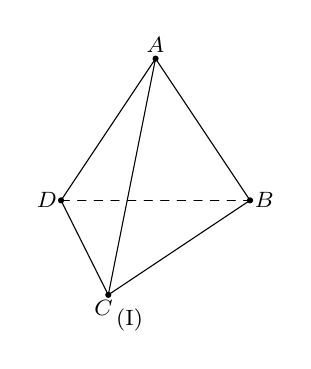
\begin{tikzpicture}[scale=0.6, font=\footnotesize,line join=round, line cap=round,>=stealth]
			\def\h{4}
			\path
			(0,0) coordinate (D)
			(1,-2) coordinate (C)
			(4,0) coordinate (B)
			(2,3) coordinate (A)
			(C)+(-50:0.7) node{(I)}
			;
			\draw
			(D)--(C)--(B)
			(A)--(B) (A)--(C) (A)--(D)
			;
			\draw[dashed] (D)--(B)
			;
			\foreach \p/\g in {A/90,B/0,C/-110,D/180}
			\draw[fill=black] (\p) circle (1.5pt)+(\g:0.3) node{$\p$};
		\end{tikzpicture}
		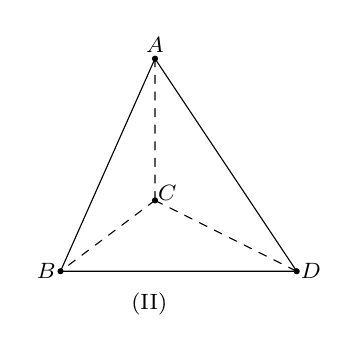
\begin{tikzpicture}[scale=0.6, font=\footnotesize,line join=round, line cap=round,>=stealth]
			\def\h{4}
			\path
			(0,0) coordinate (B)
			(2,1.5) coordinate (C)
			(5,0) coordinate (D)
			(2,4.5) coordinate (A)
			(B)+(-20:2) node{(II)}
			;
			\draw
			(A)--(B)--(D)--cycle
			;
			\draw[dashed]
			(C)--(B) (A)--(C) (C)--(D)
			;
			\foreach \p/\g in {A/90,B/180,C/30,D/0}
			\draw[fill=black] (\p) circle (1.5pt)+(\g:0.3) node{$\p$};
		\end{tikzpicture}
		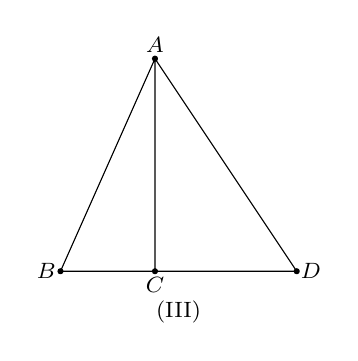
\begin{tikzpicture}[scale=0.6, font=\footnotesize,line join=round, line cap=round,>=stealth]
			\def\h{4}
			\path
			(0,0) coordinate (B)
			(2,0) coordinate (C)
			(5,0) coordinate (D)
			(2,4.5) coordinate (A)
			(C)+(-60:1) node{(III)}
			;
			\draw
			(A)--(B)--(D)--cycle
			(A)--(C)
			;
			\foreach \p/\g in {A/90,B/180,C/-90,D/0}
			\draw[fill=black] (\p) circle (1.5pt)+(\g:0.3) node{$\p$};
		\end{tikzpicture}
		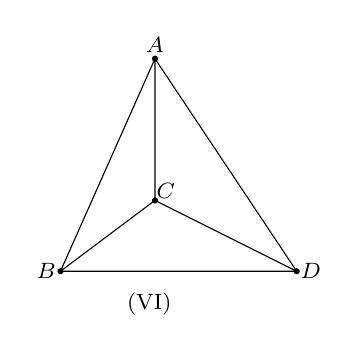
\begin{tikzpicture}[scale=0.6, font=\footnotesize,line join=round, line cap=round,>=stealth]
			\def\h{4}
			\path
			(0,0) coordinate (B)
			(2,1.5) coordinate (C)
			(5,0) coordinate (D)
			(2,4.5) coordinate (A)
			(B)+(-20:2) node{(VI)}
			;
			\draw
			(A)--(B)--(D)--cycle
			(C)--(B) (A)--(C) (C)--(D)
			;
			\foreach \p/\g in {A/90,B/180,C/40,D/0}
			\draw[fill=black] (\p) circle (1.5pt)+(\g:0.3) node{$\p$};
		\end{tikzpicture}
	\end{center}
	Hình nào có thể là hình biểu diễn của một hình tứ diện?
	\choice
	{(I)}
	{(I), (II)}
	{(I), (II), (IV)}
	{\True (I), (II), (III), (IV)}
	\loigiai{ Tất cả các hình trên đều có thể là biểu diễn của một tứ diện.
	}
\end{ex}
\begin{ex}%[1H4N2-3]
	Cho hình chóp $S.ABCD$ có đáy $ABCD$ là hình bình hành. Giao tuyến của hai mặt phẳng $(SAB)$ và $(SCD)$ là đường thẳng song song với đường thẳng nào sau đây?
	\choice
	{$BD$ }
	{$SC$}
	{$AC$}
	{\True $AB$}
	\loigiai{	
		\immini{Ta có $\heva{&S\in (SAB)\cap (SCD) \\&AB\parallel CD\\&AB\subset (SAB)\\&CD\subset(SCD)}$\\
			$\Rightarrow Sx=(SAB)\cap (SCD)\quad $(với $Sx \parallel AB\parallel CD$).}
		{	\begin{tikzpicture}[line join=round, line cap=round,thick, scale=.7]
				\coordinate (S) at (0,4);
				\coordinate (A) at (0,0);
				\coordinate (D) at (-2,-2);
				\coordinate (C) at (3,-2);
				\coordinate (B) at (5,0);
				\coordinate (E) at (-2,4);
				\coordinate (F) at (5,4);
				\draw(S)--(B) (S)--(C) (S)--(D) (B)--(C) (C)--(D) (E)--(F) node[below]{$x$};
				\draw[dashed,thin](A)--(D) (S)--(A) (A)--(B);
				\foreach \i/\g in {S/90,A/180,B/-80,C/-80,D/180}{\draw[fill=black](\i) circle (1.5pt) ($(\i)+(\g:3mm)$) node[scale=1]{$\i$};}
		\end{tikzpicture}}
	}	
\end{ex}
\Closesolutionfile{ans}
\indapan{6}{ans/ans-CTST_1-OTGK1_De2-LC}
%-------------------------------------------
\Opensolutionfile{ans}[ans/ans-CTST_1-OTGK1_De2-DS]
\cauds
\begin{ex}%[1D1N5-3]
	Cho phương trình $\sin x=m$, $m\in\mathbb{R}$. Khi đó
	\choiceTF
	{\True $\cos 2x=2m^2-1$}
	{Nếu $m=\dfrac{2}{3}$  thì  $\sin x=m$ có hai nghiệm phân biệt $x$ thuộc $[0;3\pi]$}
	{Phương trình vô nghiệm khi và chỉ khi $m>1$}
	{\True Nếu $m=\dfrac{1}{2}$ thì phương trình có nghiệm là $\hoac{&x=\dfrac{\pi}{6}+k2\pi\\&x=\dfrac{5\pi}{6}+k2\pi},\quad(k\in \mathbb{Z})$}
	\loigiai{
		\begin{itemchoice}
			\itemch Đúng. Ta có $\cos 2x=2\sin ^2x-1=2m^2-1$.
			\itemch Sai. Dựa vào hình bên dưới, ta thấy đường thẳng $y=\dfrac{2}{3}$ cắt đồ thị hàm số $y=\sin x$ trên đoạn $[0;3\pi]$ tại bốn điểm phân biệt.
			\begin{center}
				\begin{tikzpicture}[thick,>=stealth,x=1cm,y=1cm,scale=1] 
					\path
					
					(0,0) coordinate (O)
					({0.5*pi},0) coordinate (X1)
					({pi},0) coordinate (X2)
					({1.5*pi},0) coordinate (X3)
					({2*pi},0) coordinate (X4)
					({2.5*pi},0) coordinate (X5)
					({3*pi},0) coordinate (X6)
					({0.5*pi},1) coordinate (A)
					({1.5*pi},-1) coordinate (B)
					({2.5*pi},1) coordinate (C)
					(0.64,0.6) coordinate (M)
					(2.5,0.6) coordinate (N)
					(6.92,0.6) coordinate (P)
					(8.78,0.6) coordinate (Q)					
					;
					\draw[->] (-1.4,0) -- (11,0) node[below] {\small $x$};
					\draw[->] (0,-1.4)-- (0,1.8) node[right] {\small $y$};
					\draw[thick,samples=100,domain=0:10.4] plot(\x,{sin((\x)*180/pi)})node[above right] {$y=\sin x$};
					\draw(-1,0.6)-- (10,0.6) node[right] {\small $y=\dfrac{2}{3}$};
					\draw [dashed](-1,1)--(10,1) (-1,-1)--(10,-1) (X1)--(A) (X3)--(B) (X5)--(C);
					\draw  (O)node[below left]{$O$} (0,1) node[above left]{$1$} (0,-1) node[below left]{$-1$};
					\foreach \x/\g/\z in 	{X1/-90/\tfrac{\pi}{2},X2/-100/\pi,X3/-130/\tfrac{3\pi}{2},X4/-80/2\pi,X5/-90/\tfrac{5\pi}{2},X6/-90/3\pi} 
					\fill[black] (\x) circle(1pt) +(\g:5mm) node {$\z$};	
					\foreach \i in {M,N,P,Q}
					\fill[red] (\i) circle(2pt);				
				\end{tikzpicture}
			\end{center}
			Vậy nếu $m=\dfrac{2}{3}$ thì $\sin x=m\Leftrightarrow\sin x=\dfrac{2}{3}$ có bốn nghiệm phân biệt $x$ thuộc $[0;3\pi]$.
			\itemch Sai. Phương trình $\sin x=m$ vô nghiệm khi và chỉ khi $m<-1$ hoặc $m>1$.
			\itemch Đúng. Nếu $m=\dfrac{1}{2}$ thì $\sin x=m \Leftrightarrow\sin x=\dfrac{1}{2}\Leftrightarrow \sin x= \sin \dfrac{\pi}{6}\Leftrightarrow\hoac{&x=\dfrac{\pi}{6}+k2\pi\\&x=\dfrac{5\pi}{6}+k2\pi}\text{,}\quad k\in \mathbb{Z}$.
		\end{itemchoice}
	}
\end{ex}

\begin{ex}%[1D1H2-3]
	Cho  $\cot \alpha=\dfrac{7}{3}$. Khi đó
	\choiceTF
	{\True $\tan\alpha=\dfrac{3}{7}$}
	{\True $\sin^2 \alpha=\dfrac{9}{58}$}
	{Nếu $\alpha \in \left(\pi;\dfrac{3\pi}{2} \right)$ thì $\cos \alpha=\dfrac{7}{\sqrt{58}}$}
	{\True $\cos^2 \alpha- \sin ^2 \alpha=\dfrac{20}{29}$}
	\loigiai{
		\begin{itemchoice}
			\itemch Đúng. Ta có $\tan\alpha=\dfrac{1}{\cot\alpha}=\dfrac{3}{7}$
			\itemch Đúng. Ta có $\dfrac{1}{\sin ^2 \alpha}=1+\cot ^2 \alpha$, suy ra $\sin^2\alpha = \dfrac{1}{1+\cot^2 \alpha}=\dfrac{9}{58}$.
			\itemch Sai. Ta có $\cos ^2\alpha=1-\sin^2\alpha=1-\dfrac{9}{58}=\dfrac{49}{58} $. \\
			Vì $\pi<\alpha<\dfrac{3\pi}{2}$ nên $\cos \alpha<0$. Do đó $\cos \alpha=-\dfrac{7}{\sqrt{58}}$.
			\itemch Đúng. Ta biến đổi $\cos^2 \alpha- \sin ^2 \alpha= \dfrac{\cos^2 \alpha- \sin ^2 \alpha}{\cos^2 \alpha+\sin ^2 \alpha}$.\\ Vì  $\cot \alpha $ xác định nên $\sin \alpha \ne 0 $, chia cả tử và mẫu cho $\sin^2\alpha$ ta được 
			$\dfrac{\cot ^2\alpha -1}{\cot^2\alpha+1}=\dfrac{20}{29}$.
		\end{itemchoice}
	}
\end{ex}

\begin{ex} %[1D2H1-5]
	Cho dãy số $(u_n)$ biết $u_n=2^n$. Khi đó
	\choiceTF
	{Số hạng thứ $8$ của dãy số là 64}
	{Số hạng thứ $n+2$ của dãy số là $u_{n+2}=2\cdot2^n$}
	{\True Dãy số $(u_n)$ là một dãy số tăng}
	{Dãy số $(u_n)$ là dãy số bị chặn}
	\loigiai{
		\begin{itemchoice}
			\itemch Sai. Ta có $u_8=2^8=256$. Vậy số hạng thứ $8$ của dãy số là $256$.
			\itemch Sai. Ta có $ u_n=2^n\Rightarrow u_{n+2}=2^{n+2}=4\cdot2^n$.
			\itemch Đúng. Ta có $u_{n+1}-u_n=2^{n+1}-2^n=2\cdot2^n-2^n=2^n>0$, $\forall n\in \mathbb{N}^*$. \\
			Vậy dãy số $(u_n)$ là một dãy số tăng.
			\itemch Sai. Vì dãy số $(u_n)$ không bị chặn trên nên dãy số không bị chặn.
		\end{itemchoice}
	}
\end{ex}
\begin{ex}%[1H4H3-6]
	\immini {Cho tứ diện $ABCD$. Gọi $M$, $N$ lần lượt là trung điểm của $AC$ và $BC$. Trên đoạn $BD$ lấy $P$ sao cho $BP=2PD$. Khi đó
		\choiceTF
		{Gọi $I=CD \cap (MNP)$, ba điểm $I$, $N$, $P$ không thẳng hàng}
		{\True $MN\parallel (ABD)$}
		{\True Giao tuyến của hai mặt phẳng $(MNP)$ và $(ABD)$ là đường thẳng $PQ$ song song với $AB$, với điểm $Q$ thuộc đường thẳng $AD$}
		{Tứ giác $MNPQ$ là hình bình hành}
	}{
		\begin{tikzpicture}[scale=1,>=stealth, font=\footnotesize, line join=round, line cap=round]
			\coordinate (B) at (0,0);
			\coordinate (C) at (1.3,-1.3);
			\coordinate (D) at (4,0);
			\coordinate (A) at (1,3.5);
			\coordinate (M) at ($(A)!0.5!(C)$);
			\coordinate (N) at ($(B)!0.5!(C)$);
			\coordinate (P) at ($(B)!0.66!(D)$);
			\draw (A)--(B)--(C)--(D)--(A)--(C) (M)--(N);
			\draw[dashed] (B)--(D)  (N)--(P)--(M);
			\foreach \p/\r in {A/90,B/-180,C/-90,D/-50,M/180,N/180,P/90}
			\fill (\p) circle (1.5pt) node[shift={(\r:3mm)}]{$\p$};
		\end{tikzpicture}
	}
	\loigiai{
		\begin{center}
			\begin{tikzpicture}[scale=1,>=stealth, font=\footnotesize, line join=round, line cap=round]
				\coordinate (B) at (0,0);
				\coordinate (C) at (1.3,-1.3);
				\coordinate (D) at (4,0);
				\coordinate (A) at (1,3.5);
				\coordinate (M) at ($(A)!0.5!(C)$);
				\coordinate (N) at ($(B)!0.5!(C)$);
				\coordinate (P) at ($(B)!0.66!(D)$);
				\draw (A)--(B)--(C)--(D)--(A)--(C) (M)--(N);
				\draw[dashed] (B)--(D)  (P)--(M);
				\coordinate (I) at (intersection of N--P and C--D);
				\coordinate (Q) at (intersection of M--I and A--D);
				\draw (D)--(I) (M)--(I);
				\draw [dashed] (N)--(P)--(I) (Q)--(P);
				\foreach \p/\r in {A/90,B/-180,C/-90,D/-50,M/180,N/180,P/-90,I/0,Q/90}
				\fill (\p) circle (1.5pt) node[shift={(\r:3mm)}]{$\p$};
			\end{tikzpicture}
		\end{center}
		\begin{itemchoice}
			\itemch Sai. Trong mặt phẳng $(BCD)$, gọi $I=NP\cap CD$. \\
			Khi đó $\heva{& I\in CD\\& I\in NP\\& NP\subset (MNP)}\Rightarrow I=CD\cap(MNP)$.		\\
			Vì $I\in NP$ nên ba điểm $I$, $N$, $P$ thẳng hàng.
			\itemch Đúng. Vì $M$, $N$ lần lượt là trung điểm của $AC$ và $BC$ nên $MN$ là đường trung bình của $\triangle ABC$. Do đó $MN\parallel AB$. 	Mà $AB\subset(ABD)$ nên $MN\parallel (ABD)$.
			\itemch Đúng. Ta có $\heva{&P\in(MNP)\cap (ABD)\\&MN\parallel AB\\&NM\subset(MNP)\\&AB\subset (ABD)}\Rightarrow(MNP)\cap (ABD)=PQ$, (với $PQ\parallel AB\parallel MN$).
			\itemch Sai. Giả sử tứ giác $MNPQ$ là hình bình hành. Khi đó $MN\parallel PQ$ và $MN=PQ$.\\
			Vì $MN\parallel AB$ nên $\dfrac{MN}{AB}=\dfrac{1}{2}\Rightarrow MN=\dfrac{AB}{2}.\quad(1)$\\
			Vì $PQ\parallel AB$ nên $\dfrac{PQ}{AB}=\dfrac{PD}{BD}=\dfrac{1}{3}\Rightarrow PQ=\dfrac{AB}{3}.\quad(2)$\\
			Từ $(1)$ và $(2)$ suy ra $MN\ne PQ$.\\
			Do đó, tứ giác $MNPQ$ không phải là hình bình hành.\\
			Tứ giác $MNPQ$ là hình thang vì $MN\parallel PQ$.
		\end{itemchoice}
	}
\end{ex}
\Closesolutionfile{ans}
\indapan{3}{ans/ans-CTST_1-OTGK1_De2-DS}
%-------------------------------------------
\Opensolutionfile{ans}[ans/ans-CTST_1-OTGK1_De2-KQ]
\caukq
\begin{ex}%[1D1V4-8]%
	Giả sử khi một cơn sóng biển đi qua một cái cọc ở ngoài khơi, chiều cao của nước được mô hình hoá bởi hàm số $h(t)=90 \cos \left(\dfrac{\pi}{10}t\right)$, trong đó $h(t)$ là độ cao tính bằng centimét trên mực nước biển trung bình tại thời điểm $t$ giây. Tìm chiều cao của sóng (cm) (là khoảng cách theo phương thẳng đứng giữa đáy và đỉnh của sóng).\\
	\shortans{$180$}
	\loigiai{
		Ta có $-90 \leq 90 \cos \left(\dfrac{\pi}{10} t\right) \leq 90$.\\
		Suy ra chiều cao của sóng là $90- (-90) =180$ (cm).	}
\end{ex}

\begin{ex}%[1D2V2-7]
	Một kiến trúc sư thiết kế một hội trường với $15$ ghế ngồi ở hàng thứ nhất, $18$ ghế ngồi ở hàng thứ hai, $21$ ghế ngồi ở hàng thứ ba, và cứ như vậy (số ghế ở hàng sau nhiều hơn $3$ ghế so với số ghế ở hàng liền trước nó). Nếu muốn hội trường đó có sức chứa ít nhất $870$ ghế ngồi thì kiến trúc sư đó phải thiết kế tối thiểu bao nhiêu hàng ghế?\\
	\shortans{$20$}
	\loigiai{
		Số ghế ở mỗi hàng của hội trường lập thành một cấp số cộng với số hạng đầu $u_1 = 15$ và công sai $d = 3$.\\
	  Giả sử cần thiết kế tối thiếu $n$ hàng ghế để hội trường có sức chứa ít nhất $870$ ghế ngồi.\\
		Ta có $S_n=\dfrac{n}{2}\left[2 u_1+(n-1) d\right]=\dfrac{n}{2}\left[2\cdot15+(n-1)\cdot3\right]\geq 870$.\\
		Biến đổi bất phương trình này, ta được $$n(30+3 n-3) \geq 1740 \Leftrightarrow 3n^2+27n-1740 \geq 0\Rightarrow n \ge 20.$$
		Vậy cần thiết kế tối thiểu $20$ hàng ghế để thỏa mãn yêu cầu bài toán.
	}
\end{ex}
\begin{ex}%[1D2V3-8]
	Người ta thiết kế một cái tháp gồm $11$ tầng theo cách: Diện tích bề mặt trên của mỗi tầng bằng nửa diện tích mặt trên của tầng ngay bên dưới và diện tích bề mặt trên của tầng $1$ bằng nửa diện tích đế tháp. Biết diện tích đế tháp là $12\,288$ m$^2$, tính diện tích mặt trên cùng.	\\
	\shortans{$6$}
	\loigiai{
		Gọi $u_0$ là diện tích đế tháp và $u_n$ là diện tích bề mặt trên của tầng thứ $n$, với $1\le n\le 11$.\\ Theo giả thiết, ta có $u_{n+1}=\dfrac{1}{2}u_n$, $0\le n\le 10$.\\ 
		Dãy số $(u_n)$ lập thành cấp số nhân với số hạng đầu $u_0=12\,288$ và công bội $q=\dfrac{1}{2}$.\\ 
		Diện tích mặt trên cùng của tháp là $u_{11}=u_0\cdot q^{11}=12\,288\cdot{\left(\dfrac{1}{2}\right)}^{11}=6$ m$^2$.
	}
	
\end{ex}
\begin{ex}%[1H4V2-4]
	\immini[thm]{Cho hình chóp $S.ABCD$ có đáy là hình bình hành. Trên cạnh $SA$ lấy điểm $M$ sao cho $MA = 2MS$. Mặt phẳng $(CDM)$ cắt $SB$ tại $N$. Biết rằng $AB=2$, tính tổng $MN+CD$. Kết quả làm tròn đến hàng phần trăm.\\
		\shortans{$2{,}67$}}{
		\begin{tikzpicture}[scale=1,>=stealth, font=\footnotesize, line join=round, line cap=round]
			\coordinate (A) at (0,0);
			\coordinate (B) at (-1.6,-1);
			\coordinate (D) at (3.5,0);
			\coordinate (C) at ($(B)+(D)-(A)$);
			\coordinate (S) at ($(A)+(-0.7,3)$);
			\coordinate (M) at ($(A)!0.66!(S)$);
			\coordinate (N) at ($(B)!0.66!(S)$);			
			\draw (S)--(B)--(C)--(D)--cycle;
			\draw (S)--(B) (S)--(C);
			\draw[dashed] (A)--(B) (A)--(D)--(M)--(C) (S)--(A);
			\foreach \p/\r in {S/90,A/170,B/-90,C/-45,D/0,M/135}
			\fill (\p) circle (1.5pt) node[shift={(\r:3mm)}]{$\p$};
	\end{tikzpicture}}
	\loigiai{	
		\immini{
			Xét hai mặt phẳng $(MCD)$ và $(SAB)$ có $M$ là điểm chung, mà $AB \parallel CD$. Do đó giao tuyến của hai mặt phẳng $(MCD)$ và $(SAB)$ là $MN$ $(MN\parallel AB$, với $N$ thuộc $SB$).\\
			Theo định lí Ta-lét trong tam giác $SAB$, ta có $\dfrac{MN}{AB}=\dfrac{SM}{SA}=
			\dfrac{1}{3}\Leftrightarrow MN=AB\cdot\dfrac{1}{3}=\dfrac{2}{3}$.\\
			Vì $ABCD$ là hình bình hành nên $CD=AB=2$. Do đó  $MN+CD=\dfrac{2}{3}+2=\dfrac{8}{3}\approx 2{,}67$.
		}{
			\begin{tikzpicture}[scale=1,>=stealth, font=\footnotesize, line join=round, line cap=round]
				\coordinate (A) at (0,0);
				\coordinate (B) at (-1.6,-1);
				\coordinate (D) at (3.5,0);
				\coordinate (C) at ($(B)+(D)-(A)$);
				\coordinate (S) at ($(A)+(-0.7,3)$);
				\coordinate (M) at ($(A)!0.66!(S)$);
				\coordinate (N) at ($(B)!0.66!(S)$);			
				\draw (S)--(B)--(C)--(D)--cycle;
				\draw (S)--(B) (S)--(C);
				\draw[dashed] (A)--(B) (A)--(D)--(M)--(C) (S)--(A) (M)--(N);
				\foreach \p/\r in {S/90,A/170,B/-90,C/-45,D/0,M/135,N/180}
				\fill (\p) circle (1.5pt) node[shift={(\r:3mm)}]{$\p$};
			\end{tikzpicture}
		}
	}	
\end{ex}

\begin{ex}%[1D1C5-6]
	Vận tốc $v_1$ (cm/s) của con lắc đơn thứ nhất và vận tốc $v_2$ (cm/s) của con lắc đơn thứ hai theo thời gian $t$ (giây) được cho bởi các công thức:
	$$v_1(t)=-4 \cos \left(\dfrac{2 t}{3}+\dfrac{\pi}{4}\right) $$ và  $$ v_2(t)=2 \sin \left(2 t+\dfrac{\pi}{6}\right).$$
	Hãy cho biết trong khoảng thời gian $t\in [0;10]$, có bao nhiêu lần vận tốc của con lắc đơn thứ nhất gấp hai lần vận tốc của con lắc đơn thứ hai.\\
	\shortans{$6$}
	\loigiai{Thời điểm $t$ mà tại vận tốc của con lắc đơn thứ nhất gấp hai lần vận tốc của con lắc đơn thứ hai là nghiệm của phương trình: 
		\begin{eqnarray*}
			&&-4 \cos \left(\dfrac{2 t}{3}+\dfrac{\pi}{4}\right)=2\cdot2 \sin \left(2 t+\dfrac{\pi}{6}\right) \\
			&\Leftrightarrow &\cos \left(\dfrac{2 t}{3}+\dfrac{\pi}{4}\right)=-\sin \left(2 t+\dfrac{\pi}{6}\right) \\
			&\Leftrightarrow &\cos \left(\dfrac{2 t}{3}+\dfrac{\pi}{4}\right)=\sin \left(-2 t-\dfrac{\pi}{6}\right) \\
			&\Leftrightarrow &\cos \left(\dfrac{2 t}{3}+\dfrac{\pi}{4}\right) = \cos \left[\dfrac{\pi}{2}-\left(-2 t-\dfrac{\pi}{6}\right)\right]\\
			&\Leftrightarrow & \cos \left(\dfrac{2 t}{3}+\dfrac{\pi}{4}\right) = \cos \left(2 t+\dfrac{2\pi}{3}\right)\\
			&\Leftrightarrow &  \hoac{&\dfrac{2 t}{3}+\dfrac{\pi}{4}=2 t+\dfrac{2\pi}{3}+k2\pi\\&\dfrac{2 t}{3}+\dfrac{\pi}{4}=-2 t-\dfrac{2\pi}{3}+k2\pi}\text{,}  \quad k\in \mathbb{Z}\\
			&\Leftrightarrow &  \hoac{ &-\dfrac{4t}{3}=\dfrac{5\pi}{12}+k2\pi\\&\dfrac{8t}{3}=-\dfrac{11\pi}{12}+k2\pi}\text{,}  \quad k\in \mathbb{Z}\\
			&\Leftrightarrow &  \hoac{&t=-\dfrac{5\pi}{16}-k\dfrac{3\pi }{2}\quad (1)\\&t=-\dfrac{11\pi}{32}+k\dfrac{3\pi}{4} \quad (2) }\text{,}  \quad k\in \mathbb{Z}.
		\end{eqnarray*}
		Mà $t\in [0,10]$ suy ra 
		\begin{itemize}
			\item 		$(1)\Leftrightarrow 0\leq -\dfrac{5\pi}{16}-k\dfrac{3\pi }{2}\leq 10 \Leftrightarrow -\dfrac{5}{24}-\dfrac{20}{3\pi}\leq k\leq -\dfrac{5}{24}$, vì $k\in\mathbb{Z}$ nên $k\in\{-2;-1\}$. 
			Do đó có $2$ thời điểm $t_1=\dfrac{43\pi}{15}$ và $t_2=\dfrac{19\pi}{16}$.
			\item 		$(2)\Leftrightarrow 0\leq -\dfrac{11\pi}{32}+k\dfrac{3\pi}{4} \leq 10 \Leftrightarrow \dfrac{11}{24}\leq k\leq \dfrac{11}{24}+\dfrac{40}{3\pi}$, vì $k\in\mathbb{Z}$ nên $k\in\{1;2;3;4\}$. 
			Do đó có $4$ thời điểm $t_3=\dfrac{13\pi}{32}$, $t_4=\dfrac{37\pi}{32}$, $t_5=\dfrac{61\pi}{32}$ và $t_6=\dfrac{85\pi}{32}$.
		\end{itemize}
		Vậy có $6$ thời điểm xảy ra vận tốc của con lắc đơn thứ nhất gấp hai lần vận tốc của con lắc đơn thứ hai.
	}
\end{ex}
\begin{ex}%[1H4C3-4]
	Cho hình chóp $S.ABCD$ có đáy $ABCD$ là hình bình hành tâm $O$. Gọi hai điểm $M, N$ lần lượt trên các cạnh $SB, SC$ sao cho $\dfrac{SN}{SC}=\dfrac{1}{2}$ và $\dfrac{SM}{SB}=\dfrac{2}{3}$. Gọi $P$ là giao điểm của $SD$ và $(AMN)$. Tính tỉ số $\dfrac{SP}{SD}$ (kết quả làm tròn đến hàng phần trăm).\\
	\shortans{$0{,}67$}
	\loigiai{
		\immini{Trong mặt phẳng $(SAC)$, gọi $K=SO\cap AN$.\\
			Trong mặt phẳng $(SBD)$, gọi $P=SD\cap MK$. \\
			Mà $MK\subset (AMN)$ nên $P=SD\cap (AMN)$. \\
			Tam giác $SAC$ có $AN$ và $SO$ là hai đường trung tuyến nên $K$ là trọng tâm của tam giác $SAC$. Suy ra $\dfrac{SK}{SO}=\dfrac{2}{3}$. $\quad \quad (1)$\\
			Mà $\dfrac{SM}{SB}=\dfrac{2}{3}$. $ \quad \quad (2)$ \\
			Từ $(1)$ và $(2)$, suy ra $ \dfrac{SK}{SO}=\dfrac{SM}{SB}$.\\
		}{
			\begin{tikzpicture}[scale=1,>=stealth, font=\footnotesize, line join=round, line cap=round]
				\coordinate (B) at (0,0);
				\coordinate (A) at (-1.6,-1);
				\coordinate (C) at (3.5,0);
				\coordinate (D) at ($(C)-(B)+(A)$);
				\coordinate (S) at ($(A)+(1.2,4.5)$);
				\coordinate (M) at ($(S)!0.67!(B)$);
				\coordinate (N) at ($(S)!0.5!(C)$);			
				\draw(S)--(A)--(D)--(C)--(S)--(D);
				
				\draw[dashed] (A)--(B)--(C) (S)--(B) (A)--(C) (B)--(D) (A)--(M)--(N)--cycle;
				\coordinate (O) at  (intersection of A--C and B--D);
				\coordinate (K) at  (intersection of S--O and A--N);
				\coordinate (P) at  (intersection of M--K and S--D);
				\draw[dashed] (S)--(O) (M)--(P);
				\foreach \p/\r in {S/90,A/170,B/-90,C/-45,D/-30,M/135,N/100,O/-90,K/70,P/40}
				\fill (\p) circle (1.5pt) node[shift={(\r:3mm)}]{$\p$};
		\end{tikzpicture}}
		\noindent
		Theo định lí Ta-lét đảo trong tam giác $SBO$, ta có
	$KM \parallel BO$.\\
	Do đó $\dfrac{SP}{SD}=\dfrac{SK}{SO}=\dfrac{2}{3}\approx 0{,}67$.
	}
\end{ex}
\Closesolutionfile{ans}
\indapan{6}{ans/ans-CTST_1-OTGK1_De2-KQ}